% $Id$
%
% Copyright 2011, 2012, 2013, 2014; Daniel Bosk <daniel@bosk.se>
%
% This work is licensed under the Creative Commons Attribution-ShareAlike 3.0 
% Unported license.  To view a copy of this license, visit URL
%
%   http://creativecommons.org/licenses/by-sa/3.0/.
%

\documentclass[a4paper,titlepage,reqno,final,oneside]{amsbook}
%\documentclass[a4paper,titlepage,reqno,final,twoside]{amsbook}
%\documentclass[a4paper,reqno,twoside,draft]{amsbook}
\usepackage{amsbooka}
\usepackage{fixltx2e}
\usepackage[utf8]{inputenc}
\usepackage[T1]{fontenc}
\usepackage[ibycus,german,english,swedish]{babel}
\usepackage{xparse}
\usepackage{graphicx}
\usepackage[hyphens]{url}
\usepackage{lettrine}
\usepackage[strict]{csquotes}
\usepackage{setspace}
\usepackage{nomencl}
\usepackage{marginnote}
\usepackage{subfig}
\usepackage{booktabs}
\usepackage[multiple]{footmisc}
\usepackage{verbatim}
\usepackage{ifdraft}
\usepackage{asymptote}
\usepackage{datetime}

\ifdraft{%
  \usepackage{fancyhdr}
  \usepackage{showlabels}
}{%
  \if@twoside
    \usepackage[a4paper,rmargin=6cm]{geometry}
  \fi
}

\usepackage[natbib,style=alphabetic,maxbibnames=99]{biblatex}
\addbibresource{matematik-1.bib}
%\addbibresource{krypto/introcrypt.bib}
%\addbibresource{pwdanalysis/literature.bib}

\usepackage{amssymb}
\usepackage{amsmath}
\usepackage{amsthm}
\newtheorem{theorem}{Sats}[chapter]
\newtheorem{proposition}{Proposition}[chapter]
\newtheorem{lemma}{Lemma}[chapter]
\newtheorem{corollary}{Korollarium}[chapter]
\newtheorem{conjecture}{Förmodan}[chapter]
\theoremstyle{definition}
\newtheorem{axiom}{Axiom}[chapter]
\newtheorem{definition}{Definition}[chapter]
\newtheorem{example}{Exempel}[chapter]
\newtheorem{exercise}{Övning}[chapter]
\theoremstyle{remark}
\newtheorem{remark}{Anmärkning}[chapter]

\numberwithin{section}{chapter}
\numberwithin{equation}{chapter}
\numberwithin{figure}{chapter}
\numberwithin{table}{chapter}

\usepackage{varioref}
\renewcommand{\reftextbefore}{(föregående sida)}
\renewcommand{\reftextfacebefore}{(föregående sida)}
\renewcommand{\reftextafter}{(nästa sida)}
\renewcommand{\reftextfaceafter}{(nästa sida)}
\renewcommand{\reftextfaraway}[1]{(sidan~\pageref{#1})}
\usepackage{hyperref}
\usepackage[noabbrev,swedish]{cleveref}
\crefname{conjecture}{förmodan}{förmodan}
\crefname{axiom}{axiom}{axiom}
\crefname{exercise}{övning}{övning}
\Crefname{exercise}{Övning}{Övning}
\crefname{corollary}{korollarium}{korollarium}
%\crefname{proposition}{proposition}{proposition}

\renewcommand{\qedsymbol}{Q.E.D.}
\DeclareDocumentCommand{\N}{}{\ensuremath{\mathbb{N}}}
\DeclareDocumentCommand{\Z}{}{\ensuremath{\mathbb{Z}}}
\DeclareDocumentCommand{\Q}{}{\ensuremath{\mathbb{Q}}}
\DeclareDocumentCommand{\R}{}{\ensuremath{\mathbb{R}}}
\DeclareDocumentCommand{\powerset}{}{\ensuremath{\mathcal{P}}}
%\DeclareMathSymbol{\powerset}{\mathord}{MnSyC}{180}
\DeclareDocumentCommand{\U}{}{\ensuremath{\mathcal{U}}}
\DeclareDocumentCommand{\V}{}{\ensuremath{\mathcal{V}}}
\DeclareMathOperator{\card}{card}
\DeclareMathOperator{\tnot}{icke}
\DeclareMathOperator{\tor}{eller}
\DeclareMathOperator{\tand}{och}
\DeclareMathOperator{\congruent}{\equiv}


\makenomenclature{}
\makeindex{}

\includeonly{%
  frontmatter,preface,intro,logik,mangder,%
  naturliga,heltalen,talsystem,backmatter%
}

\begin{document}
\ifdraft{%
  \fancypagestyle{plain}{%
    \renewcommand{\headrulewidth}{0pt}
    \fancyhead{}
    \fancyfoot[co,ce]{\thepage}
    \fancyfoot[ro,le]{%
      \tt Draft: \today~\currenttime{}
    }
  }
  \fancypagestyle{ams}{%
    \renewcommand{\headrulewidth}{0pt}
    \fancyhead[ce]{\small\leftmark}
    \fancyhead[co]{\small\rightmark}
    \fancyhead[lo,re]{}
    \fancyhead[ro,le]{\thepage}
    \fancyfoot[ro,le]{%
      \tt Draft: \today~\currenttime{}
    }
  }
  \pagestyle{ams}
}{}

\title{%
  Matematik för alla, volym I%
}
\author{%
  Daniel Bosk%
}

\frontmatter
%\begin{abstract}
%    \input{abstract.tex}
%\end{abstract}

\ifdraft{}{%
    \if@twoside
    \newgeometry{rmargin=4cm,lmargin=4cm}
    \fi
}
\maketitle
\ifdraft{}{%
    \if@twoside
    \restoregeometry{}
    \fi
}
%\begin{titlepage}
%   \begin{center}
%       \vskip0.1\textheight
%       \textsc{\huge \...@title}
%       \vskip0.1\textheight
%       \textsc{\large \...@author}
%       \vskip0.7\textheight
%       \textsc{\...@date}
%   \end{center}
%\end{titlepage}

\cleardoublepage{}
{
    \small
    \setlength{\parskip}{0.5em}
    \setlength{\parindent}{0em}
    \vspace*{\fill}
    \input{LICENSE}
}

\tableofcontents
\cleardoublepage{}

\include{preface}

\mainmatter{}
\ifdraft{%
  \onehalfspacing{}
}{}
% main chapters
% $Id$
%
% Copyright 2011, 2012, 2013, 2014; Daniel Bosk <daniel@bosk.se>
%
% This work is licensed under the Creative Commons Attribution-ShareAlike 3.0 
% Unported license.  To view a copy of this license, visit URL
%
%   http://creativecommons.org/licenses/by-sa/3.0/.
%
\chapter{Introduktion}\label{Introduktion}
% XXX fysik, kemi använder matematiken
\lettrine{M}{atematiken har funnits} i mer än 5000 år, men började utvecklas i 
riktning mot dagens matematik först omkring 300 f.v.t.\ i antikens Grekland 
\cite{Kline1990mtf1}.
Innan dess var matematiken endast räkning, ett verktyg för att beräkna skatter 
och konstruera byggnadsverk.

Ordet matematik har enligt~\cite{OED2013maths} sitt ursprung i grekiskans 
\emph{\ibygr{ma'qhma} (m{\'a}th{\=e}ma)}, vilket betyder \emph{lärande, 
studier, vetenskap}.
Det är i det antika Grekland som dagens matematik har sitt ursprung.
De studerade främst geometri och gjorde detta genom att sätta upp några 
grundläggande antaganden, kallade postulat eller axiom, som de var övertygade 
om att de stämde överens med verkligheten.
Dessa var enkla antaganden, såsom att två parallella linjer aldrig kommer att 
skära varandra.
Utifrån dessa enkla postulat härledde de olika geometriska resultat med hjälp 
av logik och de kunde bevisa att det måste vara på ett visst sätt.
Även om de kunde se genom några enkla experiment hur saker förhöll sig till 
varandra nöjde de sig inte utan ett bevis utifrån postulaten eller tidigare 
bevisade resultat.
Anledningen till detta är enkel: för att övertyga sig om att någonting alltid 
stämmer, då räcker det inte med att testa tre fall, det räcker inte med 
hundratals fall, inte en tusentals --- dessa fall kanske avviker, eller att 
inget av dem är det specialfall som avviker.

Detta har inspirerat matematiker genom historien och är den drivkraft som 
verkat för att matematiken utvecklats till det som den är idag.
Dagens matematik bygger likt grekernas på några enkla grundantaganden som vi 
kallar för axiom.
Vidare måste begrepp som vi använder definieras tydligt för att vi exakt ska 
veta vad som menas med dem.
Detta var drivkraften bakom axiomatiseringen av de naturliga talen som vi 
kommer att se i \cref{DeNaturligaTalen}, bakom grundläggningen av de hela 
talen i \cref{ch:Heltalen}, de rationella talen i 
\cref{ch:Rationella} och de reella talen i \cref{ch:Reella}.
Länge hade matematikerna tagit talen som självklara, men vid 1800-talets mitt 
behövde de veta tydligare vad ett tal var för att kunna gå vidare.
Det som är intressant är att behovet av en axiomatisering uppstod historiskt i 
omvänd ordning av hur de logiskt är uppbyggda och presenteras i denna text.
För en detaljerad redogörelse över den historiska utvecklingen hänvisas till 
\citet{Kline1990mtf3}.

I en definition av ett objekt eller egenskap sätter vi upp regler för hur ett 
objekt som är av denna typ eller har denna egenskap ska bete sig.
Om vi kan visa att ett objekt uppfyller reglerna i definitionen, då måste
objektet också vara av den typen eller ha den egenskapen.

\begin{example}\label{ex:cykel}
  Vi använder följande definition: en \emph{cykel} har åtminstone ett hjul och 
  vevarmar med pedaler som används för att driva hjulen och ge cykeln fart.

  Om vi tittar på fordonet i \cref{fig:cykel} ser vi att det har 
  åtminstone ett hjul (det har två), det har vevaxlar med pedaler som används 
  för att driva hjulen och således ge fordonet fart.
  Alltså måste det enligt vår definition vara en cykel.
\end{example}
\begin{figure}
  % XXX create figs/cykel.eps
  \includegraphics[width=0.7\textwidth]{figs/cykel.eps}
  \caption{En illustration av en cykel.}\label{fig:cykel}
\end{figure}

\begin{example}\label{ex:bil}
  Vi använder samma definition som i \cref{ex:cykel}.
  Om vi tittat på fordonet i figur \cref{fig:sparkcykel} ser vi att det 
  har åtminstone ett hjul.
  Det saknas dock vevarmar för att driva hjulen.
  Vi kan således konstatera att en sparkcykel enligt definitionen i 
  \cref{ex:cykel} inte är en cykel.
\end{example}
\begin{figure}
  % XXX create figs/sparkcykel.eps
  \includegraphics[width=0.7\textwidth]{figs/sparkcykel.eps}
  \caption{En illustration av en sparkcykel.}\label{fig:sparkcykel}
\end{figure}

Med denna typ av definitioner kan vi veta exakt, vi kan bevisa att ett objekt 
är av en specifik typ --- likt vi gjorde i exemplen ovan.
Vi kan också göra det omvända, om ett objekt är av denna typen uppfyller det de
givna reglerna.
Exempelvis, om någon säger att de har en cykel, då måste den ha åtminstone ett 
hjul och vevarmar med pedaler som driver den framåt.
När vi bevisar saker kan vi alltså utgå från enbart dessa regler, det är detta 
som är grunden inom matematiken.


%%%%%%%%%%%%%%%%%%%%%%%%%%%%%%%%%%
% NOTATION
%%%%%%%%%%%%%%%%%%%%%%%%%%%%%%%%%%
\section{Den missförstådda algebran}

Innan vi går vidare till våra studier av matematiken ska vi ägna några rader åt 
något som i onödan förrvirrat alltför många: algebra.
Algebran har många gånger beskrivits som \enquote{att räkna med bokstäver}, 
vilket är tämligen missvisande, vi ska i detta avsnitt förklara vad algebra 
faktiskt är.

I vårt dagliga tal har vi diverse språkliga konstruktioner för att veta vilka 
objekt vi samtalar om, exempelvis \enquote{den svarta bilen närmast hitåt} 
eller \enquote{korsningen närmast skolan}.
Vi använder dessa beskrivningar utan större ansträngning.
Ibland blir det dock fel, vi har säkert alla hamnat i en situation som krävt 
uttrycket \enquote{jaha, du menar den, jag trodde att du menade något helt 
annat}.
Då måste vi förbättra noggrannheten i våra beskrivningar av objekten för att 
bli förstådda utan vidare missförstånd.

Vi kan också prata om klasser av objekt, exempelvis träd.
De flesta har säkert stött på uttrycken \enquote{en björk har löv} eller 
\enquote{björkar har löv}, \enquote{en tall har barr} eller \enquote{tallar har 
barr}.
Det är för de flesta självklart vad som menas med en björk, att det är ett träd 
av släktet björk (\emph{betula}).
Den specifika arten spelar ingen roll, exempelvis hängbjörk (\emph{betula 
pendula}) och dvärgbjörk (\emph{betula nana}) är båda björkar.
Uttryckssättet brukar användas i meningar som \enquote{en björk har vit-svart 
stam} eller \enquote{björkar har vit-svarta stammar}.

\begin{exercise}
  Prata med någon om valfritt ämne, var uppmärksam på hur ni uttrycker er för 
  att säkerställa att ni \enquote{pratar om samma sak}.
\end{exercise}

Matematiken är inte särskilt mycket konstigare än vanligt språk.
Ett av matematikens främsta verktyg är just språket, utan det skulle vi inte 
kunna uttrycka våra tankar på ett effektivt sätt.
Ett annat ovärderligt verktyg är pennan med tillhörande papper.
Detta hjälper oss dels att spara våra tankar, men framförallt att strukturera 
dem.

Säg nu att vi vill diskutera olika exotiska blommor som finns hos en 
blomsterhandlare.
Då vi själva inte är experter på exotiska blommor vet vi inte namnet på dem, så 
vi kan inte använda namnen för att diskutera dem.
Ibland kanske vi släktets namn, exempelvis orkidé (\emph{orchidaceae}), men det 
finns så många olika orkidéer att detta inte alltid hjälper.
Om alla blommor är av olika färg skulle vi kunna använda färgen för att 
identifiera de olika blommorna, exempelvis \enquote{jag tycker bäst om den 
gröna blomman}.
Men, det är sällan detta är fallet, så det är inte en hållbar metod.
En annan naturlig metod är att numrera dem, exempelvis \enquote{jag tycker bäst 
om den första blomman vi tittade på}.
Denna metod är mer hållbar.

Nu vill vi göra samma sak med papper och penna, kanske för att göra en 
inköpslista.
Då det tar mycket längre tid att skriva något än att säga samma sak, vill vi 
naturligtvis ha en kortare notation.
Vi kanske bara skriver \enquote{1:a} eller bara \enquote{1}, istället för 
\enquote{den första blomman} eller \enquote{blomma nummer ett}.
Om vi nu vill ha flera av en sort, då finns det en risk att vi förvirrar oss om 
vi skriver \enquote{2 3}.
Betyder detta att vi vill ha två av den tredje blomman eller tre av den andra 
blomman?
En bättre lösning är därför att vi hittar på namn eller symboler till de olika 
blommorna.
Vi skulle kunna rita en liten bild av de blommor vi tycker bäst om och vill 
köpa.
Detta tar dock tid, och blir inte alltid särskilt bra.
Vi kan därför använda symboler som vi redan har namn på, och som vi kan skriva 
väldigt effektivt: vårt alfabet.
Låt den första blomman vara \(a\), den andra \(b\), och så vidare.
Då finns det ingen risk att vi blandar ihop antalet med sorten likt ovan, vi 
kan skriva exempelvis \(2c\) och vet exakt vad vi menar.

Detta är bakgrunden till den matematiska notationen med bokstäver.
Det är således inget märkligt med den matematiska notationen som skrämt så 
många, det är helt enkelt ett enkelt sätt att namnge saker på ett skrivvänligt 
sätt.
En nackdel är att det finns så få bokstäver.
Därför brukar man ibland även ta till det grekiska alfabetet för att få fler 
bokstäver.
En sammanfattning av detta finns i \cref{tbl:greekalpha}.

\begin{table}
  \caption{Det grekiska alfabetet.}
  \begin{tabular}{lll}
    \textbf{Versal} & \textbf{Gemen} & \textbf{Uttal} \\
    \toprule
    \(A\) & \(\alpha\) & alfa \\
    \(B\) & \(\beta\) & beta \\
    \(\Gamma\) & \(\gamma\) & gamma \\
    \(\Delta\) & \(\delta\) & delta \\
    \(E\) & \(\epsilon\) & epsilon \\
    \(Z\) & \(\zeta\) & zeta \\
    \(H\) & \(\eta\) & eta \\
    \(\Theta\) & \(\theta\) & theta \\
    \(I\) & \(\iota\) & iota \\
    \(K\) & \(\kappa\) & kappa \\
    \(\Lambda\) & \(\lambda\) & lambda \\
    \(M\) & \(\mu\) & my \\
    \bottomrule
  \end{tabular}
  \hspace{1em}
  \begin{tabular}{lll}
    \textbf{Versal} & \textbf{Gemen} & \textbf{Uttal} \\
    \toprule
    \(N\) & \(\nu\) & ny \\
    \(\Xi\) & \(\xi\) & xi \\
    \(O\) & \(o\) & omikron \\
    \(\Pi\) & \(\pi\) & pi \\
    \(P\) & \(\rho\) & rho \\
    \(\Sigma\) & \(\sigma\) & sigma \\
    \(T\) & \(\tau\) & tau \\
    \(Y\) & \(\upsilon\) & ypsilon \\
    \(\Phi\) & \(\phi\) & phi \\
    \(X\) & \(\chi\) & khi \\
    \(\Psi\) & \(\psi\) & psi \\
    \(\Omega\) & \(\omega\) & omega \\
    \bottomrule
  \end{tabular}\label{tbl:greekalpha}
\end{table}

Oftast brukar bokstäverna väljas så att de underlättar för minnet, exempelvis 
\(b\) för blomma och \(k\) för kruka.
Sedan kan man använda subskript, exempelvis kan vi beteckna de olika blommorna 
ovan som \(b_1, b_2\) och så vidare.
Då kan vi skilja blommorna från krukorna, som vi kan benämna \(k_1, k_2\) och 
så vidare.


%%%%%%%%%%%%%%%%%%%%%%%%%%%%%%%%%%%%%
% VAD ÄR MATEMATIK?
%%%%%%%%%%%%%%%%%%%%%%%%%%%%%%%%%%%%%
\section{Vad är matematik?}
% - Skillnaden mellan matematiken och andra vetenskaper.
% - Abstrakt konstruktion som endast finns i sinnet.
% - Naturvetenskap i Sverige, filosofi i resten av världen.
%   - Sveriges störta bidrag till matematikhistorien är att vi tog död på René
%     Descartes (Touraine, 1596--Stockholm, 1650).
% - Behöver inte ha någon till synes uppenbar tillämpning, det är vackert.
%   - Pierre de Fermat (160{1,7,8}--1665), advokat, upphovsman till Fermats
%     lilla sats och Fermats stora (sista) sats.
%   - Fermat--Euler satsen är grunden för kryptosystemet när man loggar in på
%     banken via internet.
% - Demokratiskt organiserad. Alla kan bidra, ex. Fermat var advokat.
Som antyddes ovan, kan matematiken beskrivas som studiet av abstrakta 
konstruktioner.
Med abstrakta konstruktioner menar vi saker som endast finns i våra tankar, 
eller vad Platon (cirka 428--348 f.v.t.) kallade \enquote{idévärlden}.
Vi sätter upp axiomen och definitionerna, vilka vi skulle kunna kalla våra 
spelregler, och undersöker sedan vad dessa spelregler ger upphov till.

Historiskt har matematiken ofta varit sammankopplad med studiet av
verkligheten.
Vi har kunnat studera verkligheten med hjälp av matematiken genom att våra
grundregler varit grundläggande principer för verkligheten\footnote{%
  Se exempelvis Euklides postulat för geometrin i \cref{ch:Geometri} eller~\cite[kap.\ 4]{Kline1990mtf1}.
}.
Men trots detta är matematiken skild från verkligheten.
De axiom vi utgår ifrån behöver inte vara principer från verkligheten.
Det finns matematiska konstruktioner som kan te sig så verklighetsfrånkopplade
att icke-matematiker ifrågasätter varför de studeras, och detta för oss in på
ett viktigt konstaterande:
Matematiken har inte alltid studerats enbart för att kunna dra slutsatser om
verkligheten.
Många matematiker genom historien studerade matematiken enbart för den rena
matematikens skull --- för att den var vacker, inte för att den gick att
tillämpa på verkligheten.
De ville utforska den värld som spänns upp av axiomen.
Exempel på sådana är Pierre de Fermat (cirka 1607--1650) som är upphovsman till 
den kända \emph{Fermats stora sats}.
Han var advokat och amatörmatematiker.
Fermats stora sats eller \emph{Fermats sista sats} säger att ekvationen
\(x^n+y^n=z^n\), där \(x,y\) och \(z\) är heltal, saknar lösningar för heltal
\(n\) som är större än två.
Fermat lämnade en anteckning i marginalen av sin kopia av Diophantus (omkring 
år 250) bok \emph{Arithmetica} att han hade ett bevis för detta, men att 
marginalen var för liten för att rymma det.
Det tog matematiker ända fram till år 1994 att bevisa satsen, så möjligen
hade Fermat inte ett korrekt bevis då beviset som togs fram inryms på tusentals 
sidor och krävde hundratals år av matematisk utveckling.
Han hade däremot ett korrekt bevis för sin \emph{lilla sats} som säger att om
\(p\) är ett primtal, då ger \(a^{p-1}\) alltid resten \(1\) vid division med
\(p\).
(Detta tas upp i \cref{ch:Talteori}.)
Leonard Euler (1707--1783) generaliserade Fermats lilla sats till att gälla även
sammansatta tal, och denna generalisering är känd som \emph{Eulers sats} eller 
ibland \emph{Fermat--Eulers sats}.
Resultaten för dessa hade inget tillämpningsvärde för tiden, utan drivkraften
var att utforska matematikens vackra värld och finna vackra resultat som dessa.
År 1978 publicerades dock en tillämpning av satsen.
Det var Ronald Rivest (1947--), Adi Shamir (1952--) och Leonard Adleman 
(1945--) som då publicerade ett kryptosystem sedermera känt som RSA\@.
RSA-systemet bygger på Eulers sats och systemet ligger till grund för
mycket av den säkra kommunikationen som sker på internet idag.
Det dröjde alltså cirka 300 år innan någon fann en tillämpning, innan dess var 
det vara ett vackert resultat.

Detta visar även vikten av den så kallade grundforskningen, den forskning som 
inte har någon omedelbar tillämplighet, utan enbart syftar till att fördjupa 
mänsklighetens kunskap inom området.
Detta är inte viktigt bara för matematiken utan för alla vetenskaper.
För vi kan ställa oss frågan: hade vi hade haft säker kommunikation på internet
idag om vi bara utforskat det som verkat direkt tillämpbart?

%Vi ska med det gå vidare till nästa kapitel som handlar om matematikens grund
%-- logik och bevis.
%Det är logiken som är matematikens verktyg för att resonera kring de axiom som
%vi antagit.


%%%%%%%%%%%%%%%%%%%%%%%%%%%%%%%%%
% UPPLÄGG
%%%%%%%%%%%%%%%%%%%%%%%%%%%%%%%%%
%\section{Bokens upplägg}
%...
%

\ifdraft{}{%
  \part{Den matematiska grunden}
}
\chapter{Logik och bevis}%
\label{ch:Logik}
\lettrine{M}{atematiken har sin} grund i logiken.
Det är logiken som ger matematiken möjligheten till ett resonemang och
möjligheten till härledning.
Matematiken utgår från några få grundläggande antaganden, kallade \emph{axiom}, 
från vilka matematiska resultat härleds.
En matematiker nöjer sig således inte med att undersöka några exempel --- eller
göra experiment --- inte ens tusen- eller miljontals exempel duger.
Det är detta som skiljer matematiken från exempelvis fysiken och kemin, trots
att dessa till mycket stor omfattning använder matematiken som hjälpmedel.
Vi känner nämligen inte till alla grundläggande principer för fysiken och 
kemin, utan det är (återstoden av) dessa vi försöker att finna genom 
grundforskningen inom dessa ämnen.
Vi känner däremot till alla grundläggande principer för matematiken, detta för
att matematiken är skapad av oss --- det är vi som bestämt dessa principer.
I detta kapitel ska vi lära oss mer om dessa.


%%%%%%%%%%%%%%%%%%%%%%%%%%%%%%%%%%
% LOGIK
%%%%%%%%%%%%%%%%%%%%%%%%%%%%%%%%%%
\section{Logik}

All matematisk argumentation består av \emph{utsagor}.
Utsagor\index{utsaga} är deklarativa meningar som kan klassificeras som 
antingen \emph{sanna} eller \emph{falska}.
Vi behöver inte alltid veta precis vilket, men det måste vara den ena eller den
andra --- aldrig båda.
Detta kallas inom logiken för \emph{lagen om det uteslutna tredje}\index{lagen 
om det uteslutna tredje}.
Om vi tittar på följande meningar:
\begin{enumerate}
  \item Denna text är skriven på svenska.
  \item Grön är en fin färg.
  \item Denna mening är falsk.
  \item Det finns oändligt många primtalstvillingar.
  \item \(x^2+1=0\)
\end{enumerate}

Den första meningen är en utsaga, och den är sann.
Den andra är ej en utsaga i logisk bemärkelse, det är en smaksak.
Den tredje meningen är ej en utsaga, den kan varken vara sann eller falsk
eftersom att det leder till motsägelsefulla slutsatser.
Den fjärde meningen är en utsaga, ingen vet dock om den är sann eller falsk.
Den femte och sista symbolföljden är en utsaga, men vi vet inte vad \(x\) är så
vi kan inte uttala oss om den skulle vara sann eller falsk.
Detta visar vikten av att tydligt specificera alla delar av en utsaga, så att
det är alldeles klart vad vi menar.
Den femte utsagan skulle behöva ändras till exempelvis \enquote{det finns ett
komplext tal \(x\) sådant att \(x^2+1=0\)} för att den skulle vara sann.
Om vi istället ändrat den till \enquote{det finns ett heltal \(x\) sådant att
\(x^2+1=0\)} skulle den vara falsk oavsett hur vi väljer \(x\) eftersom att
det inte finns ett sådant heltal.  En utsaga som alltid är falsk kallar vi för 
\emph{motsägelse}\index{motsägelse!utsaga} eller
\emph{kontradiktion}\index{kontradiktion|see {motsägelse}}.
En utsaga som alltid är sann kallar vi för \emph{tautologi}\index{tautologi}.

Två utsagor \(P\) och \(Q\) sägs vara logiskt 
ekvivalenta\index{ekvivalens!logisk} om \(P\) är sann
precis när \(Q\) är sann och följaktligen om \(P\) är falsk precis när \(Q\)
är falsk.
Vi skriver detta som \(P\equiv Q\).

\subsection{Kombinerade utsagor}

Vi vill också kunna forma nya utsagor från redan kända, detta genom att
kombinera och modifiera dem.
Om \(P\) är en utsaga, då säger vi att \emph{negationen}\index{negation!logisk} 
av \(P\), betecknad \(\lnot P\) eller \(\tnot P\), är falsk precis när \(P\) är 
sann och sann precis när \(P\) är falsk.
Vi kommer då fram till \emph{lagen om dubbelnegation}\index{lagen om 
dubbelnegation}.
Om vi funderar på vad som händer om vi tar \(\lnot(\lnot P)\) så kommer vi
fram till att \(P\equiv \lnot(\lnot P)\).
\begin{example}
  Ett exempel på negation, låt \(P\) vara utsagan \enquote{vi befinner oss i
  Sverige}.
  Då blir \(\lnot P\) \enquote{vi befinner oss inte i Sverige}.
  Vi kan också se att \(\lnot(\lnot P)\) blir \enquote{att vi inte befinner oss 
  inte i Sverige}, vilket är lite svårare att läsa men resulterar i att vi 
  måste befinna oss i Sverige.
\end{example}
\begin{example}
  Vi kan också titta på följande utsaga, \enquote{alla svenskar tycker om
  surströmming}.
  Negationen av den utsagan är \emph{inte} att ingen svensk tycker om
  surströmming, utan den är \enquote{inte alla svenskar tycker om 
  surströmming}.
  Det räcker då med att det finns en svensk som inte tycker om
  surströmming --- detta är en viktig skillnad att inte ta fel på!
\end{example}

Vi kan också kombinera utsagor genom \emph{konjunktioner}\index{konjunktion}.
Om \(P\) och \(Q\) är utsagor, då betecknar vi konjunktionen som \(P\tand Q\)
eller \(P\land Q\).
Konjunktionen är sann då både \(P\) och \(Q\) båda är sanna och falsk annars.
\begin{example}\label{ex:KonjunktionInternet}
  Låt \(P\) vara utsagan \enquote{jag bor i Sverige} och \(Q\) vara utsagan 
  \enquote{jag har en internetuppkoppling}.
  Då kan vi skapa den nya utsagan \(P\land Q\) som blir \enquote{jag bor 
    i Sverige \emph{och} jag har en internetuppkoppling}.
\end{example}

\begin{exercise}
  När är de olika utsagorna \(P\), \(Q\) och \(P\land Q\) i
  \cref{ex:KonjunktionInternet} sanna respektive falska?
\end{exercise}

Vi har också \emph{disjunktionen}\index{disjunktion} som betecknas \(P\tor Q\) 
eller \(P\lor Q\).
Disjunktionen är sann om antingen \(P\) eller \(Q\) eller båda är sanna, och är
således falsk endast när \(P\) och \(Q\) båda är falska.
\begin{example}
  Julfika kräver lussebullar \emph{eller} julfika kräver pepparkakor.
  Denna utsaga säger att om vi fikar lussebullar, då är det julfika.
  Den säger också att det är julfika om vi fikar pepparkakor.
  Den säger också att det är julfika om vi fikar både lussebullar och 
  pepparkakor samtidigt.
\end{example}

Konjunktionen och disjunktionen sammanfattas i en sanningstabell i
\cref{tbl:SanningKonjunktionDisjunktion}.

\begin{table}
  \caption{%
    Sanningstabell för konjunktionen och disjunktionen.
    S betecknar sant och F betecknar falskt.
  }
  \begin{tabular}{cccc}
    \(P\)  & \(Q\)   & \(P\land Q\)  & \(P\lor Q\) \\
    \toprule
    S      &  S      & S             & S \\
    S      &  F      & F             & S \\
    F      &  S      & F             & S \\
    F      &  F      & F             & F \\
    \bottomrule
  \end{tabular}\label{tbl:SanningKonjunktionDisjunktion}
\end{table}

\begin{exercise}\label{xrc:tartkalas}
  Vilken av följande logiska utsagor passar bäst för ett tårtkalas?
  På ett kalas
  \begin{enumerate}
    \item äts tårta \emph{och} dricks saft \emph{och} äts kakor
      \emph{och} dricks kaffe \emph{och} dricks te.
    \item äts tårta \emph{eller} dricks saft \emph{eller} äts kakor
      \emph{eller} dricks kaffe \emph{eller} dricks te.
  \end{enumerate}
\end{exercise}

\begin{exercise}
  Ingen av utsagorna i \cref{xrc:tartkalas} är egentligen riktigt bra 
  utsagor för att avgöra om något är ett tårtkalas.
  \begin{enumerate}
    \item Diskutera bristerna i de olika utsagorna.
    \item Utforma en egen bättre utsaga.
  \end{enumerate}
\end{exercise}

Hittills har vi kombinerat konjunktioner med konjunktioner och disjunktioner 
med disjunktioner, men det går naturligtvis även att kombinera konjunktioner 
med disjunktioner.
Vi visar här ett exempel på detta.

\begin{example}\label{ex:aldersgrans}
  I Sverige är åldersgränserna för film följande: under 7 år, under 11 år och 
  under 15 år~\cite{aldersgranser}.
  En film som inte får ses av barn under 11 år får ses av barn som uppfyller 
  följande utsaga: barnet är minst 11 år \emph{eller} barnet är minst 7 år 
  \emph{och} i vuxens sällskap.
  Notera att vi här kombinerat tre utsagor, först med disjunktion och sedan med 
  konjunktion.
\end{example}

\begin{exercise}
  Du kanske märkte av ett problem med utsagan i \cref{ex:aldersgrans}, om 
  inte kommer du att uppmärksamma det nu.
  Utsagan i exemplet har följande form: \(P\lor Q\land R\).
  Undersök om det spelar någon roll om vi tar \(P\lor Q\) eller \(Q\land R\) 
  först, det vill säga om \(P\lor (Q\land R)\equiv (P\lor Q)\land R\).
\end{exercise}

\begin{exercise}
  Testa att kombinera negationer, konjunktioner och disjunktioner, går det
  att forma några logiskt ekvivalenta utsagor?
\end{exercise}

\subsection{Implikationer}

Implikation är synonymt med ordet 
\emph{medför}\index{implikation}\index{medför|see {implikation}}.
Om \(P\) och \(Q\) är utsagor säger vi att \(P\) \emph{implicerar} \(Q\) eller
\emph{om \(P\), då \(Q\)}.
Vi ska undersöka när denna sammansatta utsaga bör vara sann och när den bör
vara falsk.
Låt oss formulera ett exempel.
\begin{example}
  Låt \(P\) vara utsagan \enquote{jag vinner pengar} och \(Q\) vara utsagan
  \enquote{jag köper nya böcker till skolan}.
  Utsagan \(P\implies Q\) blir då \enquote{\emph{om} jag vinner pengar,
  \emph{då} köper jag nya böcker till skolan}.
\end{example}
Implikationen är uppenbart falsk om jag vinner pengar men inte köper böcker till
skolan, men sann om jag köper böcker.
Annars, om jag inte vinner pengar, då har jag heller inte lovat att köpa
böcker till skolan.
Då måste utsagan vara sann i det fallet.
Men att jag inte vinner pengar hindrar mig ju inte att köpa böcker till
skolan ändå, följaktligen borde utsagan vara sann även i det fallet.
Det är detta resonemang som gjort att sanningsvärdena för implikationen är 
valda som de är.
Implikationens olika sanningsvärden sammanfattas i den vänstra delen av 
\cref{tbl:SanningImplikation}.

Vi kan naturligtvis vända på implikationen, om \(P\) och \(Q\) är utsagor och
\(P\implies Q\) då säger vi att dess \emph{invers}\index{invers!logisk} är 
\(Q\implies P\).
Inversen för en implikation är inte nödvändigtvis logiskt ekvivalent med
implikationen.
Ett exempel får illustrera.
\begin{example}\label{ex:kontrapositiv}
  Låt \(P\) vara utsagan \enquote{vi är i Stockholm} och \(Q\) vara utsagan 
  \enquote{vi är i Sverige}.
  Då blir \(P\implies Q\) utsagan \enquote{om vi är i Stockholm, då är vi i
  Sverige}.
  Dess invers \(Q\implies P\), \enquote{om vi är i Sverige, då är vi i
  Stockholm}, är däremot inte sann eftersom att vi skulle kunna vara i
  exempelvis Sundsvall, Göteborg eller Kiruna som också är städer i Sverige.

  Om vi däremot tittar på utsagan \(\lnot Q\implies \lnot P\), det vill säga
  \enquote{om inte vi är i Sverige, då är vi inte i Stockholm}, ser vi att 
  denna måste vara sann samtidigt som \(P\implies Q\).
\end{example}
Den senare utsagan i \cref{ex:kontrapositiv}, \(\lnot Q\implies \lnot P\), 
kallas för den \emph{kontrapositiva}\index{kontrapositiv!utsaga} utsagan av 
\(P\implies Q\).

Om \(P\implies Q\) och \(Q\implies P\) båda skulle vara sanna, vilket ibland är 
fallet, då skriver vi detta som \(P\iff Q\).
Utsagan \(P\iff Q\) kallas för 
\emph{dubbelimplikation}\index{dubbelimplikation|see {logisk ekvivalens}} eller
\emph{ekvivalens}\index{ekvivalens!logisk} och är sann då \(P\) och \(Q\) båda 
är sanna och då de båda är falska.
Den utläses som \emph{\(P\) om och endast om \(Q\)}\index{om och endast om|see 
{logisk ekvivalens}}.
\enquote{Om och endast om} förkortas ibland som \enquote{omm}.
Vi kan se att \(\iff\) får samma betydelse som \(\equiv\).

\begin{exercise}
  Undersök några olika logiska utsagor, likt den kontrapositiva utsagan, och se 
  om du kan finns några intressanta ekvivalenser.
\end{exercise}

Vi ska nu avsluta med en viktig logisk ekvivalens till implikationen.
Denna ligger till grund för motsägelsebevis.
Utsagan \((P\land\lnot Q)\implies C\), där \(C\) är en motsägelse och
därmed alltid är falsk, är logiskt ekvivalent med \(P\implies Q\).
Detta ses tydligast i en sanningstabell, och den är given i
\cref{tbl:SanningImplikation} tillsammans med implikationen och dess
kontrapositiva utsaga.
Implikationen \(P\implies Q\) är bara falsk när \(P\) är sann och \(Q\) är
falsk.
Konjunktionen \(P\land\lnot Q\) är sann endast när \(P\) är sann och \(Q\) är
falsk.
Om \(C\) alltid är falsk, då kommer \(P\land\lnot Q\implies C\) att vara falsk
endast när \(P\land\lnot Q\) är sann.
Men det är ju precis när \(P\) är sann och \(Q\) är falsk, det vill säga när
\(P\implies Q\) är falsk.
Följaktligen måste de vara logiskt ekvivalenta.

\begin{table}
  \caption{%
    Sanningstabell för implikationen och dess logiskt ekvivalenta former.
    S betecknar sant och F betecknar falskt.
  }
  \begin{tabular}{ccccccc}
    \(P\) &
    \(Q\) &
    \(P\implies Q\) &
    \(\lnot(P\land \lnot Q)\) &
    \(\lnot Q\implies \lnot P\) &
    \(C\) & \((P\land\lnot Q)\implies C\) \\
    \toprule
    S & S & S & S & S & F & S \\
    S & F & F & F & F & F & F \\
    F & S & S & S & S & F & S \\
    F & F & S & S & S & F & S \\
    \bottomrule
  \end{tabular}\label{tbl:SanningImplikation}
\end{table}


%%%%%%%%%%%%%%%%%%%%%%%%%%%%%%%%%%
% AXIOM, SATSER OCH BEVIS
%%%%%%%%%%%%%%%%%%%%%%%%%%%%%%%%%%
\section{Axiom, satser och bevis}

För att det ska kunna gå att härleda någonting måste det finnas
några grundläggande utsagor som en grund att bygga på.
Dessa utsagor kallar vi för \emph{axiom}\index{axiom}, och det är från dessa
alla matematiska härledningar utgår.
Vi har också definitioner som indirekt kan specificera axiom.

Vi har ovan redan sett några axiom, nämligen de logiska axiomen.
Det vill säga sanningstabellerna vi tittat på ovan, de fungerar som axiom för 
logiken.
Vi var dock inte tydliga med att dessa var axiom eftersom att vi inte visste 
vad ett axiom var då.
Vi ska i kommande kapitel ta upp de matematiska axiomen.
Det finns axiom som används i nästan all matematik, dessa är axiomen för
mängdläran (\cref{ch:Mangder}), och det finns olika axiomuppsättningar 
inom specifika områden inom matematiken.
Exempelvis ska vi se en axiomuppsättning för geometri 
i \cref{ch:Geometri}, denna gäller för klassisk geometri, det vill säga 
geometri i plana ytor.
I sfärisk geometri, geometri på ytan av en rund boll, som vi inte tar upp 
i denna volym, byts några av axiomen ut.

Grunden må vara viktig att stå på, men möjligheten att ta oss vidare till nya 
resultat --- satser --- är också av yttersta vikt.
Faktum är ju att vi tidigare behövde logiken för att kunna resonera och dra
slutsatser, för att kunna bevisa nya resultat.
Nya resultat, som är implikationer eller dubbelimplikationer, sammanfattas i
något som kallas för \emph{satser}\index{sats}.
En sats ges oftast på formen \enquote{om dessa villkor \(P\) är uppfyllda, då 
gäller även \(Q\)}, där \(P\) och \(Q\) är utsagor.
Men en sats kan inte bara presenteras utan vidare, den kräver alltid ett
\emph{bevis}\index{bevis}.
Ett bevis är en logisk härledning som utgår från axiomen och andra tidigare
bevisade satser för att visa att om \(P\) är sann då måste även \(Q\) vara sann
precis då.
Det vill säga visa att implikationen är sann.

Satsen är huvudbegreppet, men vi har även andra typer av satser.
Vi har \emph{lemman}\index{lemma}, som är hjälpsatser\index{hjälpsats}.
De är också satser, men av mindre betydelse.
Dessa behöver vi för att visa ett mindre resultat för att beviset för en annan
sats inte ska bli onödigt långt.
Vi har även \emph{korollarier}\index{korollarium}, som är
följdsatser\index{följdsats}.
Detta är satser som följer mer eller mindre direkt från en annan sats och har
därför ett mycket kort bevis.

Vi ska nu titta på några vanliga bevismetoder.
När ett bevis genomförs och presenteras brukar detta avslutas med 
\textsc{Q.E.D.}, som är en förkortning för latinets \emph{Quod Erat
Demonstrandum} och betyder \enquote{vilket skulle visas}.
Detta är ett arv från tiden då latin var det vetenskapliga språket och mer
eller mindre all vetenskaplig kommunikation skedde på latin.
Det skulle kunna jämföras med engelskans position idag.

Vi kommer nedan att beskriva den bakomliggande idén för respektive bevismetod.
Därefter kommer vi att se dem tillämpas i resterande kapitel i boken.

\subsection{Motexempelbevis}

Vi börjar med den enklaste bevismetoden.
Om någon skulle påstå att \enquote{alla svenskar tycker om surströmming}, då 
räcker det med att vi hittar en svensk som inte tycker om surströmming för att
motbevisa påståendet.
Det vill säga, vi hittar ett motexempel\index{motexempelbevis}.
Kom ihåg från tidigare att negationen av utsagan \enquote{alla svenskar tycker 
om surströmming} är \enquote{det finns åtminstone en svensk som inte tycker om
surströmming} och att det är denna utsaga som vi bevisar genom att finna en
sådan svensk.

\subsection{Direkta bevis}

Vi låter \(P\) och \(Q\) vara utsagor.
För att \emph{hypotesen}\index{hypotes} \(P\) ska implicera 
\emph{konklusionen}\index{konklusion} \(Q\) måste \(P\) vara sann
precis när \(Q\) är sann.
Vi åstadkommer detta genom konstruktionen av en kedja av implikationer
\[
  P\implies R_1, R_1\implies R_2, \ldots, R_n\implies Q.
\]
Enligt \emph{lagen om syllogism}\index{lagen om syllogism} måste då \(P\implies 
Q\).
Karakteristiskt för denna bevismetod är att det bara är att \enquote{jobba på} 
för att komma fram till konklusionen.

\begin{exercise}
  Övertyga dig själv med hjälp av sanningstabeller
  \begin{enumerate}
    \item att \(P\implies R_1\) och \(R_1\implies R_2\) och \(R_2\implies Q\) 
      är ekvivalent med \(P\implies R_1\implies R_2\implies Q\), därefter
    \item att \(P\implies Q\) är ekvivalent med \(P\implies R_1\implies 
      R_2\implies \cdots\implies Q\).
  \end{enumerate}
\end{exercise}

\subsection{Kontrapositiva bevis}

Låt \(P\) och \(Q\) vara utsagor.
Eftersom att vi tidigare, i \cref{tbl:SanningImplikation}, sett att den
kontrapositiva\index{kontrapositivt!bevis} implikationen \(\lnot Q\implies\lnot 
  P\) är logiskt ekvivalent
med \(P\implies Q\) kan vi likväl bevisa den kontrapositiva implikationen som
\(P\implies Q\).
Vi vill kunna göra detta för att ibland kan det vara lättare att visa än \(P\) 
medför \(Q\).

\subsection{Motsägelsebevis}

Motsägelsebeviset\index{motsägelse!bevis} och det direkta beviset är kanske de 
bevismetoder som används flitigast i denna bok.
Motsägelsebeviset är effektivt och kan ofta vara enklare att använda än att
konstruera ett direkt bevis.
Metoden använder en logisk ekvivalens, precis som föregående metod, nämligen att
\((P\land\lnot Q)\implies C\) är logiskt ekvivalent med \(P\implies Q\) när
\(C\) är en motsägelse.
Den säger att vi ska anta vår hypotes \(P\) och även anta motsatsen
\(\lnot Q\) till vår önskade konklusion \(Q\).
Om dessa antaganden tillsammans leder till en utsaga som alltid är falsk, det
vill säga en motsägelse \(C\), då har vi visat att \(P\) implicerar \(Q\)
eftersom att detta är logiskt ekvivalent.


\section{Fördjupande läsning}

För vidare läsning om logik, se exemeplvis bilaga A i \emph{Introduction to 
real analysis} av \citet{Bartle2000itr} eller, för ytterligare fördjupning, del 
A i \emph{Foundations of logic and mathematics} av 
\citet{nievergelt2002foundations}.


\include{mangder}
\ifdraft{}{%
  \part{Tal och aritmetik}
}
\include{naturliga}
\include{heltalen}
\chapter{Talteori}%
\label{ch:Talteori}%\nocite{Laksov2005kou,Bartle2000itr}
\lettrine{T}{alteori är studiet} av talen, primärt de hela talen.
Ett exempel på ett mycket enkelt talteoretiskt fynd är att vartannt tal är 
jämnt och vartannat är udda; det vill säga att varje heltal \(n\) kan skrivas 
som \(n = 2k\) om det är jämnt respektive \(n = 2k+1\) om det är udda, där 
\(k\) är ett heltal.

Enligt en redogörelse av \citet{Kline1990mtf1} inleddes studiet av talen redan 
av babylonierna\footnote{%
  Babylonier är en benämning av de folk som levde i området Mesopotamien, ett 
  område mellan floderna Eufrat och Tigris i vad som idag är 
  Irak~\cite{Kline1990mtf1}.
}, vars storhetstid var mellan cirka 2500--300 f.v.t.\@
De härledde bland annat resultatet att \[1 + 2 + 4 + \cdots + 2^n = 2^n + (2^n 
- 1) = 2^{n+1} - 1.\]
% XXX Ge exempel på Pythagoreiska tripplar: a^2 + b^2 = c^2
% XXX Ta upp Diophantos
Grekerna fortsatte i sin tur att studera talen under sin storhetstid, vilken 
varade mellan cirka 600 f.v.t.\ till omkring år 300.
De mest kända grekiska matematiker och filosofer som studerade talteori är 
kanske Pythagoras\index{Pythagoras} (cirka 585--500 f.v.t.), då främst 
gemensamt med sina anhängare kända som Pythagoréerna\index{Pythagoréerna}, samt 
Euklides\index{Euklides} (omkring 300 f.v.t.).
Anledningen till att saker tillskrivs Pythagoréerna är för att de historiska 
dokument som finns tillgängliga inte skiljer på vad som åstadkommits av 
Pythagoras själv eller hans lärljungar, därför används Pythagoras och 
Pythagoréerna synonymt i de flesta texter (denna inräknad).

Bland Pythagoréernas resultat kan nämnas att
\begin{equation}
  \label{eq:pyth-square}
  n^2 + (2n + 1) = (n + 1)^2.
\end{equation}
Anledningen till detta resultat var att Pythagoréerna representerade tal som 
prickar i sanden, se figurerna~\ref{fig:pyth-triangles} 
och~\ref{fig:pyth-squares}.
\begin{figure}
  \centering
  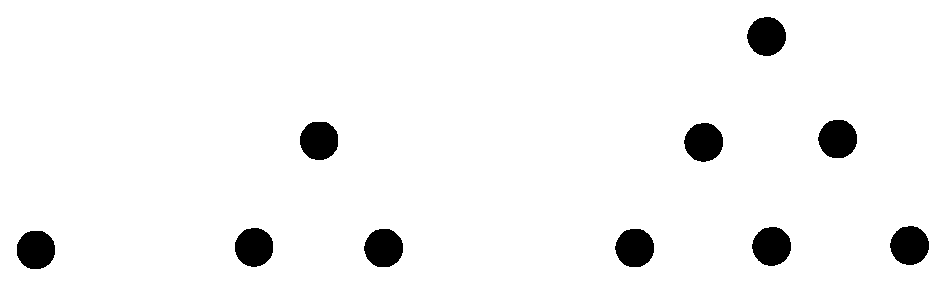
\includegraphics[width=4cm]{figs/pyth-triangles.eps}
  \caption{%
    Talen 1, 3 och 6 representerade med Pythagoreiska trianglar.
  }\label{fig:pyth-triangles}
\end{figure}
\begin{figure}
  \centering
  
\includegraphics[width=4cm]{figs/pyth-squares.eps}
  \caption{%
    Talen 1, 4 och 9 representerade med Pythagoreiska kvadrater.
  }\label{fig:pyth-squares}
\end{figure}
Tal som kunde representeras som en triangel kallade de följaktligen för 
triangulära tal\index{triangulära tal} och tal som kunde representeras som 
kvadrater kallades för kvadratiska tal\index{kvadratiska tal}.
Ett resultat som fascinerade dem var att varje kvadratiskt tal kunde 
konstrueras genom additionen av två triangulära tal.
Ett annat, det som gavs som \cref{eq:pyth-square} ovan, är hur nästa 
kvadratiska tal återfinns; \( (n+1)^2 \) är det kvadratiska tal som följer 
\(n^2\) och \(2n + 1\) är antalet prickar som måste läggas till längs kanterna.
\begin{exercise}
  Undersök om det finns ett liknande uttryck för triangulära tal.
\end{exercise}
\begin{exercise}
  För vilka triangulära tal gäller att om två triangulära tal adderas är 
  resultatet ett kvadratiskt?
\end{exercise}

Fermats och Eulers resultat som omnämndes redan i \cref{Introduktion} är ett 
mycket intressant talteoretiskt resultat.
Det är fortfarande historiskt, dock modernt i jämförelse med ovan nämnda 
resultat.
Vi kommer att behandla Fermats och Eulers satser senare i detta kapitel.

Ytterligare ett resultat, ett olöst sådant, är Goldbachs förmodan.
Denna förmodan uttalades av Chrisitan Goldbach (1690--1794)~\cite{goldbach} och 
säger att varje naturligt tal kan skrivas som en summa av primtal.
Begreppet primtal är centralt för talteorin och vi kommer strax att återkomma 
till dessa.


%%%%%%%%%%%%%%%%%%%%%%%%%%%%%%%%%%%%%%%%%%%%
% DELBARTHET
%%%%%%%%%%%%%%%%%%%%%%%%%%%%%%%%%%%%%%%%%%%%
\section{Delbarhet}
Ett av de centrala begreppen inom talteorin är delbarheten hos de hela 
talen.
Vi inleder avsnittet med att definiera vad vi menar med detta.
\begin{definition}[Delbarhet]\index{delbarhet}\index{delare}\index{äkta delare}
  Vi säger att ett tal \(a\in\Z\) delar ett tal \(b\in\Z\) om det finns ett tal 
  \(q\in\Z\) sådant att \(b = qa\).
  Vi skriver då \(a\mid b\), vilket utläses som \emph{\(a\) delar \(b\)}.
  På motsvarande sätt har vi \(a\nmid b\) för \emph{\(a\) delar inte \(b\)}.
  Om dessutom \(a\neq b\) sägs \(a\) vara en \emph{äkta delare} till \(b\).
\end{definition}
\begin{example}
  Vi har att \(2\mid 4\) eftersom att \(4 = 2\cdot 2\), två är dessutom en äkta 
  delare.
  Tre är däremot inte en delare till fyra, så \(3\nmid 4\).
  Vi har att \(3\mid 12\) eftersom att \(12 = 3\cdot 2^2\), tre är dessutom en 
  äkta delare till \(12\).
  Vi har har \(12\mid 12\) eftersom att \(12 = 1\cdot 12\), men \(12\) är dock 
  inte en äkta delare till \(12\).
\end{example}
\begin{exercise}\label{xrc:delare}
  Undersök hur olika tal delar varandra och se om ni finner något samband.
\end{exercise}

För att underlätta i kommande bevis ger vi först ett antal fundamentala lemman 
om egenskaperna för delbarhet.
\begin{lemma}\label{lem:divtransitiv}
  Om \(a\mid b\) och \(b\mid c\), då måste även \(a\mid c\).
\end{lemma}
\begin{proof}
  Låt \(b = xa\) och \(c = yb\), då måste \(c = yxa\) och följaktligen måste 
  \(a\mid c\).
\end{proof}
\begin{lemma}\label{lem:divassoc}
  Om \(a\mid b\) och \(a\mid c\), då måste \(a\mid xb + yc\) för alla heltal 
  \(x\) och \(y\).
\end{lemma}
\begin{exercise}
  Bevisa \cref{lem:divassoc}.
\end{exercise}
\begin{lemma}\label{lem:divdistnondiv}
  Om \(a\mid b\) och \(a\nmid c\), då måste \(a\nmid b+c\).
\end{lemma}
\begin{exercise}
  Bevisa \cref{lem:divdistnondiv}, ett förslag är att tillämpa 
  \cref{lem:divassoc}.
\end{exercise}
\begin{exercise}
  Diskutera och förklara varför \(3\mid 6\) men \(3\nmid 5\), \(3\nmid 2\) och 
  \(3\nmid 1\) då \(6 = 5 + 1 = 4 + 2 = 3 + 2 + 1 = 3 + 3\).
\end{exercise}
\begin{lemma}\label{lem:divnoll}
  Om \(ab\neq 0\) och \(a\mid b\) och \(b\mid a\), då måste \(a = b\) eller \(a 
  = -b\).
\end{lemma}
\begin{proof}
  Låt \(a = xb\) och \(b = ya\), då måste \(b = yxb\).
  Eftersom att \(b\neq 0\) måste \(yx = 1\) och således är \(x\) och \(y\) 
  antingen båda \(1\) eller båda \(-1\).
\end{proof}
\begin{lemma}\label{lem:divneg}
  Om \(a\mid b\), då måste \(-a\mid b\), \(-a\mid -b\) och \(a\mid -b\).
\end{lemma}
\begin{exercise}
  Bevisa \cref{lem:divneg}.
\end{exercise}
\begin{exercise}
  Diskutera innebörden av de olika lemmorna.
\end{exercise}

När vi nu är bekanta med begreppet delare ska vi introducera 
divisionsalgoritmen.
Denna ger oss ett verktyg för att dela heltal med varandra och är faktiskt den 
första typen av division som introduceras i svensk skola, den introduceras 
redan i årskurs 1--3 i grundskolan.

\begin{theorem}[Divisionsalgoritmen]\label{thm:divisionsalgoritmen}\index{divisionsalgoritmen}
  Låt \(b\) vara ett positivt heltal.
  För varje heltal \(a\) finns unika heltal \(q\) och \(r\) sådana att \[a = qb 
  + r,\] där \(0\leq r < b\).
\end{theorem}

Innan vi bevisar att algoritmen är korrekt är det lämpligt att vi bevisar ett 
antal lemman.

\begin{lemma}\label{lem:DisjunktaIntervallAvZ}
  Låt \( i_x = \{y\in\Z \colon xb\leq y < (x + 1)b\} \) beteckna ett intervall 
  för varje \(x\in\Z\).
  Då är \(i_x\) och \(i_{x'}\) disjunkta, det vill säga \(i_x\cap \i_{x'} = 
    \emptyset\).
  Deras union \(\cup_{x\in \Z} i_x = \Z\) utgör hela \(\Z\).
\end{lemma}
\begin{exercise}
  Bevisa ovanstående lemma.
  Arbeta med de två delarna var för sig: bevisa att intervallerna är disjunkta 
  och bevisa att unionen utgör hela \(\Z\).
\end{exercise}

\begin{proof}[Bevis för divisionsalgoritmen]
  Eftersom att intervallerna \[
    i_x = \{y\in\Z \colon xb\leq y < (x + 1)b\}
  \] för alla \(x\in\Z\) är disjunkta och deras union \(\cup_{x\in \Z} i_x = 
    \Z\) utgör hela \(\Z\) (\cref{lem:DisjunktaIntervallAvZ}) måste det finnas 
  ett heltal \(q\) sådant att \(qb\leq a < (q+1)b\).
  Låt \(r = a - qb\), då får vi från \(qb\leq a < (q + 1)b\) att \[ r = a - qb 
  < (q + 1)b - qb = b.\]

  För att visa att \(q\) och \(r\) är unika antar vi att det existerar något 
  \(q^\prime\neq q\) och något \(r^\prime\neq r\) sådana att \(a = q^\prime 
  b + r^\prime\).
  Då måste \[0 = (qb + r) - (q^\prime b + r^\prime) = (q - q^\prime)b + (r 
  - r^\prime)\] och således \[ (q - q^\prime)b = -(r - r^\prime) = r^\prime 
  - r.\]
  Följaktligen har vi att \(b\) delar \(r^\prime - r\), men detta är omöjligt 
  då \(0\leq r, r^\prime < b\) ger \(-b < r - r^\prime < b\).
  Vi har då visat att \(r = r^\prime\) och \(q = q^\prime\) och således att 
  \(q\) och \(r\) är unika.
\end{proof}

\begin{definition}
  Vi kallar \(q\) och \(r\) i \cref{thm:divisionsalgoritmen} för
  \emph{heltalskvoten till \(a\) vid division med \(b\)} respektive
  \emph{resten till \(a\) vid division med \(b\)}.
\end{definition}

Notera att enligt våra definitioner stämmer det överens att ett tal \(a\) delar 
ett tal \(b\) då resten är noll.

\begin{exercise}\label{xrc:KvotenMindre}
  Bevisa följande.
  Låt \(a\) och \(b\) vara två heltal.
  Heltalskvoten \(q\) till \(a\) vid division med \(b\) är strikt mindre än 
  \(a\) om \(b\) är strikt större än ett.
\end{exercise}
\begin{exercise}
  Visa att om \(a^2 = 4q + r\) är \(r\) lika med noll eller ett.
\end{exercise}

%%%%%%%%%%%%%%%%%%%%%%%%%%%%%%%%%%%%%%%%%%%%
% PRIMTAL OCH SAMMANSATTA TAL
%%%%%%%%%%%%%%%%%%%%%%%%%%%%%%%%%%%%%%%%%%%%
\subsection{Primtal och sammansatta tal}
Det självklara steget för den nyfikne efter att vi definierat delare är att 
undersöka vilka tal som delar varandra (\cref{xrc:delare}).
Detta har fascinerat matematiker sedan tusentals år tillbaka.
Vi vet redan att både Pythagoréerna och Euklides studerat detta.
Vi ska därför fortsätta genom att definiera ytterligare ett fundamentalt 
begrepp.
\begin{definition}\index{primtal}\index{sammansatt tal}
  Ett tal \(p > 2\) större än två vars enda positiva delare är \(1\) och \(p\) 
  sägs vara ett \emph{primtal}.
  Om \(p\) har fler delare kallas det för ett \emph{sammansatt tal}.
\end{definition}

Följande sats, aritmetikens fundamentalsats, visades i princip av Euklides.
I den sjunde boken av hans \emph{Elementa} finns två satser som tillsammans
kan visa aritmetikens fundamentalsats.
Den visades dock först i sin helhet av Carl Friedrich Gauss (1777--1855) i sin
bok tillika doktorsavhandling \emph{Disquisitiones 
  Arithmeticae}~\cite{Kline1990mtf3}, som är latin för \emph{utforskning av
tal}.
Gauss skrev boken 1798 när han var 20 år gammal och den publicerades 1801.
Den handlar om talteori och sammanfattar tidigare resultat, men introducerar
även nya.
Aritmetikens fundamentalsats var ett av dessa nya resultat.
\begin{theorem}[Aritmetikens 
  fundamentalsats]\label{thm:AritmetikensFundamentalsats}\index{aritmetikens 
    fundamentalsats}
  Ett heltal \(n\in\Z\) kan skrivas som en unik produkt av primtal och \(1\)
  eller \(-1\).
\end{theorem}
%\begin{proof}
%  % XXX Komplettera med bevis för Aritmetikens fundamentalsats
%  \dots
%\end{proof}
\begin{exercise}
  Beviset kan delas upp i två delar.
  Bevisa först att varje tal antingen är ett primtal eller kan skrivas som en 
  produkt av primtal.
  Detta görs enklast med ett induktionsbevis.
  Bevisa därefter att om ett tal kan skrivas som en produkt av primtal, då är 
  den produkten unik sånär som på ordningen av faktorerna\footnote{%
    Det vill säga \(a\cdot b\) och \(b\cdot a\) räknas som samma produkt.
  }.
  Antag att \(p_1p_2\dotsb p_m = q_1q_2\dotsb q_n\), bevisa att \(m = n\) och 
  att varje \(p_i\) motsvarar ett \(q_j\).
\end{exercise}

Följande sats har varit känd under väldigt lång tid, den är idag känd som
Euklides sats.
Eventuellt var satsen känd även tidigare, men den skrevs ned av Euklides i
den nionde boken av \emph{Elementa}.
Euklides \emph{Elementa} bestod av totalt 13 böcker och användes som lärobok
i matematik ända fram till 1900-talet.
\begin{theorem}[Euklides sats]\index{Euklides sats}
  Det finns oändligt många primtal.
\end{theorem}
\begin{proof}
  Vi antar att det finns ändligt många primtal, då kan vi beteckna mängden av 
  alla primtal som \(P = \{p_1, p_2, \dotsc, p_n\}\).
  Vi tittar på ett heltal \(m\).
  Enligt aritmetikens fundamentalsats, 
  \cref{thm:AritmetikensFundamentalsats}, kan vi välja detta \(m\) sådant 
  att \(m = p_1\cdots p_n\) är produkten av alla primtal.
  Vi låter dessutom \(q=m+1\).
  Eftersom att \(q > p_i\) för alla \(i\) kan inte \(q\) vara ett element i
  \(P\), och därför är \(q\) inte ett primtal.
  Då finns det igen enligt aritmetikens fundamentalsats ett primtal \(p\) som 
  delar \(q\).
  Eftersom att \(p\) är ett primtal måste enligt vårt antagande \(p = p_j\) för 
  något \(j\), och alltså måste \(p\) dela \(m\).
  Men om \(p\) delar både \(m\) och \(q = m + 1\), då måste \(p\) även dela
  \(q - m = 1\).
  Då detta är omöjligt får vi en motsägelse och det måste alltså finnas
  oändligt många primtal.
\end{proof}


\section{Fermats och Eulers satser}\label{sec:fermateuler}
% XXX Skriv avsnitt om Fermats och Eulers satser
[Avsnittet är ej ännu färdigskrivet.]

\begin{theorem}[Fermats lilla sats]\index{Fermats lilla sats}
  Låt \(p\) vara ett primtal.
  För alla heltal \(a\) som ej är delbara med \(p\) har vi att resten till 
  \(a^{p-1}\) vid division med \(p\) är \(1\).
\end{theorem}
\begin{proof}
  % XXX Komplettera bevis för Fermats lilla sats
  \dots
\end{proof}

\begin{exercise}
  Låt \(p\) vara ett primtal.
  Visa att för alla \(a < p\) mindre än \(p\) har vi att resten till \(a^p\) 
  vid division med \(p\) är \(a\).
\end{exercise}

\begin{definition}
  % XXX Ange definition för största gemensamma delare
  Största gemensamma delare \dots
\end{definition}
\begin{definition}
  % XXX Ange definition för relationen relativt prima
  Relativt prima \dots
\end{definition}

\begin{theorem}[Eulers sats]\index{Eulers sats}
  Låt \(n\) vara ett positivt heltal.
  För varje tal \(a\) sådant att \(a\) och \(n\) är relativt prima har vi att 
  \[ a^{\phi(n)} \congruent 1 \pmod n. \]
\end{theorem}
\begin{proof}
  % XXX Komplettera bevis för Eulers sats
  \dots
\end{proof}


\section{Stora problem inom talteorin}

Fermats stora sats, eller Fermats förmodan, ställde Fermat upp år 1637.
Han påstod sig ha ett elegant bevis, men att detta inte rymdes i marginalen där 
han skrev kommentaren.
Satsen ges här som sats istället för förmodan då den bevisades 1995 av Andrew 
Wiles (1953--).

\begin{theorem}[Fermats förmodan]\index{Fermats förmodan}\index{Fermats stora 
    sats|see{Fermats förmodan}}
  Det finns inga heltal \(a\), \(b\) och \(c\) sådana att \(a^n + b^n = c^n\) 
  för något heltal \(n\) större än två.
\end{theorem}

Då Wiles bevis är betydligt längre än denna text i sin helhet återges inte 
beviset här.
Dessutom krävs det många års universitetsstudier i matematik för att kunna 
tillgodogöra sig det.

Ett annat stort problem, men som fortfarande saknar bevis, är \emph{Goldbachs 
förmodan}.
Som nämndes i inledningen ställdes denna förmodan upp av Goldbach under 
1700-talet.
\begin{conjecture}[Goldbachs förmodan]\index{Goldbachs förmodan}
  Varje naturligt tal kan skrivas som en summa av primtal.
\end{conjecture}
En enklare version av Goldbachs förmodan bevisades år 2013, det resultatet 
säger att alla udda tal kan skrivas som en summa av primtal.

Nu till några begrepp som vi fått från Fermat och Marin Mersenne (1588--1648).
\begin{definition}
  Ett tal på formen \(F_n = 2^{2^n} + 1\) kallas för ett \emph{Fermattal}.
  Ett tal på formen \(M_p = 2^p - 1\), där \(p\) är ett primtal kallas för ett 
  \emph{Mersennetal}.
  När \(M_p\) i sin tur är ett primtal kallas det för ett 
  \emph{Mersenneprimtal}.
\end{definition}
Fermat hävdade att alla Fermattal är primtal.
Han hade dock inget bevis och det visar sig att det enbart är de fyra första 
som är primtal, det femte visade Euler att det är ett sammansatt tal.
Det är enbart dessa fyra Fermattal som vi känner till som är primtal, det är 
okänt om det finns några fler~\cite{Laksov2005kou}.
\begin{conjecture}
  Det finns oändligt många Fermattal.
\end{conjecture}
Det finns däremot desto fler kända Mersenneprimtal, vi vet dock inte om det 
finns oändligt många.
\begin{conjecture}
  Det finns oändligt många Mersenneprimtal.
\end{conjecture}

Låt oss nu gå vidare till en annan typ av tal som också fascinerat matematiker 
genom tiderna, nämligen perfekta tal.
\begin{definition}
  Ett heltal \(n\) sägs vara ett \emph{perfekt tal}\index{perfekt tal} om \(n\) 
  är summan av alla sina äkta positiva delare.
\end{definition}
\begin{example}
  Talet \(6\) är ett perfekt tal då \(6 = 3\cdot 2\cdot 1 = 3 + 2 + 1\).
\end{example}

Euler bevisade åtminstone ett resultat om perfekta tal, det ges som följande 
sats.
\begin{theorem}
  Alla jämna perfekta tal \(n\) kan skrivas på formen \(p(p + 1)/2\), där \(p\) 
  är ett Mersenneprimtal.
\end{theorem}
Det finns dock mycket som vi inte vet om perfekta tal.
Följande två hypoteser är fortfarande varken bevisade eller motbevisade.
\begin{conjecture}
  Det finns inga udda perfekta tal.
\end{conjecture}
\begin{conjecture}
  Det finns oändligt många perfekta tal.
\end{conjecture}

För vidare fördjupning inom området talteori rekommenderas
Laksovs \citetitle{Laksov2005kou}~\cite{Laksov2005kou} eller
Shoups \citetitle{ShoupNTB}~\cite{ShoupNTB}.

\chapter{Rationella tal}%
\label{ch:Rationella}
%Grekerna.
%Pythagoréerna och studiet av musik.
[Ej ännu färdigskrivet.]

\include{reella}
\include{talsystem}
\ifdraft{}{%
  \part{Ekvationer}
}
\chapter{Ekvationer}
\label{ch:Ekvationer}
\dots

\chapter{Olikheter}
\label{ch:Olikheter}
\dots

\chapter{Potensekvationer}
\label{ch:Potensekvationer}
\dots

\ifdraft{}{%
  \part{Geometri}
}
\chapter{Klassisk geometri}
\label{ch:Geometri}
\dots

\chapter{Trigonometri}
\label{ch:Trigonometri}
\dots

\chapter{Linjär algebra}
\label{ch:LinjarAlgebra}
\dots

\ifdraft{}{%
  \part{Samband och förändring}
}
\chapter{Procent och andra relativa storheter}
\label{ch:Procent}
\dots

\chapter{Olika former av förändring}
\label{ch:Forandring}
\dots

\ifdraft{}{%
  \part{Kombinatorik, sannolikhet och statistik}
}
% Copyright 2013, 2014, 2015, 2016; Daniel Bosk <daniel@bosk.se>
%
% This work is licensed under the Creative Commons Attribution-ShareAlike 4.0 
% Unported license.  To view a copy of this license, visit URL
%
%   http://creativecommons.org/licenses/by-sa/4.0/.
%

\chapter{Grundläggande kombinatorik}
\label{GrundläggandeKombinatorik}
% XXX Skriv kapitlet om kombinatorik
\lettrine{K}{ombinatorik handlar} om studiet av diskreta strukturer.
Den gren av kombinatoriken som vi ska behandla i detta kapitel är 
\emph{uppräknelig kombinatorik}.
\index{kombinatorik}
\dots

\begin{lemma}[Additionsprincipen]
\label{Additionsprincipen}
\index{additionsprincipen}
  Låt \(u_1, \dots, u_n\) vara \(n\) disjunkta mängder.
  Då är kardinaliteten \(|u_1\cup \cdots\cup u_n| = |u_1| + \cdots + |u_n|\).
\end{lemma}
\begin{proof}
  \dots
\end{proof}

\begin{lemma}[Multiplikationsprincipen]
\label{Multiplikationsprincipen}
\index{multiplikationsprincipen}
  Låt \(u_1, \dots, u_n\) vara \(n\) mängder.
  Då är kardinaliteten \(|u_1\times \cdots\times u_n| = |u_1|\cdots |u_n|\).
\end{lemma}
\begin{proof}
  \dots
\end{proof}

\begin{definition}[Permutation]
\label{Permutation}
\index{permutation}
  \dots
\end{definition}

\begin{theorem}[Antalet permutationer]
\label{AntaletPermutationer}
  \dots
\end{theorem}
\begin{proof}
  \dots
\end{proof}

\begin{definition}[Kombination]
\label{Kombination}
\index{kombination}
  \dots
\end{definition}

\begin{theorem}[Antalet kombinationer]
\label{AntaletKombinationer}
  \dots
\end{theorem}
\begin{proof}
  \dots
\end{proof}

\begin{theorem}[Dirichlets lådprincip\footnote{Även 
    duvhålsprincipen}]
\label{thm:ladprincipen}
\index{Dirichlets lådprincip}
\index{lådprincipen}
\index{duvhålsprincipen}
  % XXX Beskriv Dirichlets lådprincip
  \dots
\end{theorem}
\begin{proof}
  \dots
\end{proof}


\section{Om val}
Vi stöter ofta på val av olika slag.
Vi ska i detta avsnitt reflektera över antalet möjliga utfall som kan uppstå
genom att olika val kombineras samman.

Vi inleder med definitioner av de begrepp vi kommer att använda.

\begin{definition}\label{def:Val}
  Med \emph{val} menas att det finns \(n \geq 1\) antal distinkta alternativ
  att välja mellan, av dessa alternativ måste ett och endast ett väljas.
  Det alternativ som väljs sägs vara \emph{utfallet av valet}.
\end{definition}

Vi fortsätter med ett väldigt enkelt lemma om förhållandet mellan valets
antal alternativ och det möjliga antalet utfall.

\begin{lemma}\label{lem:AntalUtfall}
  Ett val från \(n\) alternativ har \(n\) möjliga utfall.
\end{lemma}
\begin{proof}
  För varje alternativ behövs åtminstone ett utfall.
  Om vi har \(n\) alternativ och antar att vi har \(n+1\) utfall,
  då måste det enligt Dirichlets lådprincip, \cref{thm:ladprincipen}, vara 
  något alternativ som får fler än ett utfall.
  Men om ett och samma alternativ har flera utfall, då måste dessa utfall
  vara samma utfall.
  Detta är en motsägelse och därför måste vi ha exakt \(n\) utfall.
\end{proof}

För fullständighet inkluderas även följande exempel.
\begin{example}\label{ex:Fikabrod}
  Du ska välja fikabröd till eftermiddagsfikat.
  De alternativ du har att välja mellan är en nybakad bulle, en torr kaka och
  att inte ta något fikabröd.
  Notera att välja \emph{ingenting} utgör ett alternativ, det går alltså inte
  att avstå från ett val.

  Valet av fikabröd har tre alternativ, enligt \cref{lem:AntalUtfall}
  finns således tre möjliga utfall.
  Ett utfall är att vi väljer bullen, ett annat att vi väljer kakan och det
  sista att vi väljer att inte ta något fikabröd.
\end{example}

\subsection{Att välja bland val}
Då är det dags att utöka våra möjligheter att välja genom att kombinera flera
val till ett sammansatt val.

\begin{definition}
  När ett val ska göras följt efter ett annat säger vi att vi har ett
  \emph{sammansatt val}.
  Ett sammansatt val kan ibland kallas för val.
  Varje ingående val kallas för ett \emph{delval}.
\end{definition}

\begin{example}
  Det är dags för eftermiddagsfika igen.
  Du ska först välja om du ska dricka kaffe, te eller vatten.
  (Att inte välja någonting är inte ett alternativ i detta val, detta är ett
  rent teoretiskt val eftersom att rent praktiskt finns ju alltid
  alternativet att inte fika alls.)
  Därefter ska du välja fikabröd enligt \cref{ex:Fikabrod}.
  Då har vi ett sammansatt val bestående av två delval, ett för dryck och ett
  för fikabröd.
\end{example}
\begin{exercise}
  Visa att detta stämmer överens med att välja mellan alternativen \emph{kaffe 
  och bulle}, \emph{kaffe och kaka}, \emph{te och bulle}, och så vidare.
\end{exercise}

Det är nu intressant att veta hur många möjliga utfall som ett sådant val
möjligen kan ha.
Detta sammanfattas i följande sats.

\begin{theorem}[Multiplikationsprincipen]\label{thm:Multiplikationsprincipen}
  Ett sammansatt val av \(m\) antal delval, där delval \(i\) har \(n_i\)
  antal alternativ,
  har \(n_1\cdot n_2\cdots n_m\) antal möjliga utfall.
\end{theorem}

\begin{proof}
  Låt oss börja med att titta på det sista valet, val \(m\).
  Detta val har \(n_m\) alternativ och således \(n_m\) utfall enligt
  \cref{lem:AntalUtfall}.
  Vi går vidare till valet innan, det vill säga val \(m-1\).
  Detta val har \(n_{m-1}\) möjliga utfall.
  För varje utfall av detta val kan vi få \(n_m\) utfall i val \(m\).
  Då har vi alltså tillsammans
  \begin{equation}\label{eq:MultprincipTvaVal}
    \sum_{k=1}^{n_{m-1}} n_m = \underbrace{n_m + n_m + \cdots
    n_m}_{n_{m-1}} = n_{m-1}\cdot n_m.
  \end{equation}
  För varje utfall av delval \(m-2\) kan vi få antalet utfall från
  \cref{eq:MultprincipTvaVal}.
  Det vill säga
  \begin{equation}
    \sum_{k=1}^{n_{m-2}} n_{m-1}\cdot n_m = n_{m-2}\cdot n_{m-1} \cdot n_m.
  \end{equation}
  Vi fortsätter på detta vis till vi når det första valet då vi får
  \begin{equation}
    \sum_{k=1}^{n_1} n_2\cdot n_3\cdots n_{m-2}\cdot n_{m-1}\cdot n_m
      = n_1\cdot n_2\cdots n_m,
  \end{equation}
  vilket visar satsen.
\end{proof}

Från \cref{thm:Multiplikationsprincipen} följer direkt ett enkelt resultat
som vi ger i detta korollarium\footnote{%
  Det vill säga en följdsats.
}.

\begin{corollary}\label{cor:SammansattValKonstAlternativ}
  Ett sammansatt val av \(m\) antal delval där varje delval har \(n\)
  alternativ, har \(n^m\) antal möjliga utfall.
\end{corollary}

\begin{proof}
  Om vi har ett sammansatt val av \(m\) antal delval, där delval
  \(i\) har \(n_i\) alternativ.
  Då har vi enligt \cref{thm:Multiplikationsprincipen} att det totala
  utfallet är \(n_1\cdot n_2\cdots n_m\).
  Men eftersom att alla val hade samma antal alternativ, nämligen \(n\), då
  får vi att \(n_1\cdot n_2\cdots n_m = n\cdot n\cdots n = n^m\).
  Följaktligen får vi \(n^m\) antal möjliga utfall då vi har \(m\) delval där
  varje delval har \(n\) alternativ.
\end{proof}



\section{Val av lösenord}
Vi ska nu titta på hur detta kan användas för att undersöka säkerheten hos
lösenord.
Det finns flera angreppssätt för att skapa lösenord, exempelvis genom att
välja en kombination av tecken (bokstäver, siffror och specialtecken) eller att
helt enkelt välja några ord.
Det går också att skapa lösenord genom att slumpmässigt välja några ord som
kombineras till ett lösenord.

Vi börjar med det första fallet, där vi skapar ett lösenord genom att kombinera
tecken.
Om vi ska skapa ett lösenord som är fem tecken långt och får innehålla
bokstäverna A-Z, både gemener och versaler,
siffrorna 0-9 samt
specialtecknen ''!@.\%\&'',
då kan vi se valet av lösenord som ett sammansatt val bestående av fem delval,
där alternativen för varje delval är de tillåtna tecknen.
Antalet alternativ är således \(26\cdot 2 + 10 + 5 = 67\).
Eftersom att alla delval har samma antal alternativ kan vi använda
\cref{cor:SammansattValKonstAlternativ} för att ta reda på antalet möjliga
utfall, det vill säga antalet möjliga lösenord.
Antalet lösenord som uppfyller detta krav är \(67^5 = 1350125107\).

Nu fortsätter vi med att titta på fallet med att välja lösenord genom att
slumpmässigt välja några ord.
Vi bestämmer oss för att använda ett lösenord med fyra slumpmässigt valda
ord från svenska språket.
Enligt Svenska Akademin \citep{SAOL} innehåller Svenska Akademins Ordlista
ungefär 125000 ord.
Detta ger enligt \cref{cor:SammansattValKonstAlternativ}
\begin{equation}\label{eq:AntalUtfallOrd}
  125000^4 = (2^3\cdot 5^6)^4
    = 2^{12}\cdot 5^{24}
    = 2^{12}\cdot 25^{12},
\end{equation}
det vill säga \(244140625000000000000\), möjliga lösenord.

Det senaste fallet kan också ses ur det första fallets perspektiv.
Låt oss anta att medellängden av orden vi väljer från är fem tecken och att
dessa tecken enbart är gemener.
Det innebär att vi får
\begin{equation}\label{eq:AntalUtfallTecken}
  (29^5)^4 = 29^{20} = 176994576151109753197786640401
\end{equation}
möjliga lösenord.

Hur spelar denna representation någon roll, vad betyder skillnaden mellan
\cref{eq:AntalUtfallOrd} och \cref{eq:AntalUtfallTecken}?
Det första som bör påpekas är att i \cref{eq:AntalUtfallTecken} tas även
teckenkombinationer som ej är svenska ord med.
Detta eftersom att valet var att välja fyra uppsättningar av fem tecken.
Betydelsen av detta är att om vi låter en dator bara slumpa fram 20 bokstäver
(gemener), då kommer det att resultera i antalet gissningar från
\cref{eq:AntalUtfallTecken}.
Det är inte ens säkert att datorn kommer att hitta rätt lösenord om vi råkade
välja fyra långa ord som alla var minst sex bokstäver långa.
Detta är ett problem med denna uppskattning.
Om vi däremot har en ordlista som datorn väljer ord från för att kombinera
dessa till ett lösenord om fyra ord för att gissa lösenordet, då kommer antalet
gissningar att maximalt bli \cref{eq:AntalUtfallOrd}.
Även denna metod kräver naturligtvis att orden i lösenordet finns med i
ordlistan som datorn har tillgång till.


%\include{pwdanalysis/pwdinclude}
% Copyright 2016; Daniel Bosk <daniel@bosk.se>
%
% This work is licensed under the Creative Commons Attribution-ShareAlike 4.0 
% Unported license.  To view a copy of this license, visit URL
%
%   http://creativecommons.org/licenses/by-sa/4.0/.
%

\chapter{Sannolikhetsteori}
\label{ch:Sannolikhet}
\dots

\begin{definition}[Utfall]
  Ett \emph{utfallsrum} är en uppräknelig icke-tom mängd.
  Elementen i utfallsrummet kallas \emph{utfall}.
  En \emph{händelse} är en delmängd till utfallsrummet.
\end{definition}

\begin{definition}[Sannolikhetsmått]
  \dots
\end{definition}

\begin{definition}[Sannolikhetsrum]
  \dots
\end{definition}

\begin{theorem}[Sannolikhet för händelse och komplement]
  \dots
\end{theorem}

\begin{theorem}[Sannolikhet för två händelser]
  \dots
\end{theorem}

\begin{definition}[Parvis disjunkta händelser]
  \dots
\end{definition}

\begin{definition}[Betingad sannolikhet]
  \dots
\end{definition}

\begin{definition}[Oberoende händelser]
  \dots
\end{definition}

\begin{theorem}[Bayes sats]
  \dots
\end{theorem}

\chapter{Statistikteori}
\label{ch:Statistik}
\dots

%\include{krypto/krypto}

% appendices
\appendix
\ifdraft{%
  \doublespacing{}
}{}
\chapter{Studiehandledning för Matematik 1c}\label{Studiehandledning}
%\nocite{Tobin2005msl}

\lettrine{K}{ursen Matematik 1c}
är enligt ämnesplanen 100 poäng, det vill säga att den ska ges 100 
lektionstimmar.
Dessa lektionstimmar ska fördelas på de fem huvudområden som ges under rubriken
\emph{Centralt innehåll} i ämnesplanen: 
\begin{itemize}
  \item taluppfattning, aritmetik och algebra;
  \item geometri;
  \item samband och förändring;
  \item sannolikhet och statistik; samt
  \item problemlösning.
\end{itemize}

I planeringen given nedan avser tidsåtgången lärargenomgångar, till exempel
tid när läraren går igenom innehåll vid tavlan.
Denna tid innefattar inte elevers egna arbete, redovisningar av uppgifter,
klassrumsdiskussioner etcetera.

Avsnittet \emph{Problemlösning}, som innehåller punkterna
\begin{itemize}
  \item Strategier för matematisk problemlösning inklusive användning av
    digitala medier och verktyg,
  \item Matematiska problem av betydelse för privatekonomi, samhällsliv och
    tillämpningar i andra ämnen, och
  \item Matematiska problem med anknytning till matematikens kulturhistoria,
\end{itemize}
kan med fördel inkluderas i undervisningen som tar upp övriga områden och
behöver således inte behandlas specifikt.

Inledande i kursen bör vara grundläggande logik\footnote{%
  Från området \emph{Geometri} har vi punkten \enquote{Matematisk argumentation 
    ned hjälp av grundläggande logik inklusive implikation och ekvivalens samt 
    jämförelser med hur man argumenterar i vardagliga sammanhang och inom 
    naturvetenskapliga ämnen}.
}, begreppen definition och axiom samt sats och bevis\footnote{%
  Från området \emph{Geometri} har vi punkten \enquote{Illustration av 
    begreppen definition, sats och bevis, till exempel med Pythagoras sats och 
    triangelns vinkelsumma}.
}.
Detta eftersom att dessa fundamentala begrepp är det som bygger upp
matematiken.
Därefter kan grundläggande mängdlära gås igenom, med axiom och grundläggande
satser, och konstruktionen av de naturliga talen kan visas för att visa hur
matematiken fundamentalt är uppbyggd.
För detaljer se \cref{tbl:inledning}.

\begin{table}
  \caption{%
    Planering för inledningen.
  }\label{tbl:inledning}
  \begin{tabular}{ll}
    Innehåll & Tidsåtgång (timmar) \\
    \toprule
    Logik, definition, sats och bevis. & 2 \\
    \midrule
    Mängder. & 1 \\
    \midrule
    Mängden av naturliga tal. & 1 \\
    \bottomrule
    & 4 \\
  \end{tabular}
\end{table}

Därefter följer lämpligen avsnittet \emph{Taluppfattning, aritmetik
och algebra} eftersom att taluppfattning, aritmetik och algebra är nödvändiga
för vidare studier av matematiken, och alltså nödvändiga för resten av kursen,
samt att det är naturligt att studera heltalen efter de naturliga talen.
För detaljer se \cref{tbl:talteori}.
%Eftersom att avsnittet har fem punkter bör \emph{25 timmar} avsättas för hela
%detta område.

\begin{table}
  \caption{%
    Planering för avsnittet \emph{Taluppfattning, aritmetik och
    algebra}.
  }\label{tbl:talteori}
  \begin{tabular}{ll}
    %\textbf{Innehåll} & \textbf{Tidsåtgång (timmar)} \\
    Innehåll & Tidsåtgång (timmar) \\
    \toprule
    Generalisering av aritmetikens räkneregler till att\\
      hantera algebraiska uttryck. & 2 \\
    \midrule
    Egenskaper hos mängden heltal, olika talbaser samt\\
      begreppen primtal och delbarhet. & 5 \\
    \midrule
    Egenskaper hos mängderna rationella tal, irrationella\\
      tal och reella tal. & 5 \\
    \midrule
    Begreppet linjär olikhet. & 1 \\
    \midrule
    Algebraiska och grafiska metoder för att lösa linjära\\
      ekvationer, olikheter och potensekvationer. & 5 \\
    \midrule
    Metoder för beräkningar inom vardagslivet och\\
      karaktärsämnena med reella tal skrivna på olika\\
      former, inklusive potenser med reella exponenter\\
      samt strategier för användning av digitala verktyg.
      & * \\
    \bottomrule
    & 21 \\
  \end{tabular}
\end{table}

Efter egenskaperna hos heltal, rationella och irrationella tal och algebra kan
funktionsbegreppet introduceras.
Funktionsbegreppet är ett centralt begrepp inom all matematik och bör gås
igenom tidigt i kursen för att kunna användas senare, exempelvis när
de trigonometriska funktionerna och logaritmfunktionen introduceras.
För detaljer se \cref{tbl:funktioner}.

\begin{table}
  \caption{%
    Planering för avsnittet \emph{Samband och förändring}.
  }\label{tbl:funktioner}
  \begin{tabular}{ll}
    Innehåll & Tidsåtgång (timmar) \\
    \toprule
    Begreppen funktion, definitions- och värdemängd samt\\
      egenskaper hos linjära funktioner samt potens-\\
      och exponentialfunktioner. Representationer av\\
      funktioner i form av ord, funktionsuttryck, tabeller\\
      och grafer.  & 6 \\
    \midrule
    Skillnader mellan begreppen ekvation, olikhet, algebraiskt\\
      uttryck och funktion. & 2 \\
    \midrule
    Fördjupning av procentbegreppet: promille, ppm och\\
      procentenheter. & 2 \\
    \midrule
    Begreppen förändringsfaktor och index samt metoder för\\
      beräkning av räntor och amorteringar för olika typer\\
      av lån. & 4 \\
    \bottomrule
    & 14 \\
  \end{tabular}
\end{table}

Då föregående avsnitt \emph{Samband och förändring} avslutas med
procentbegreppet är det lämpligt att fortsätta med detta i avsnittet
\emph{Sannolikhet och statistik}.
Procentbegreppet används då i en annan form än som ett mått av förändring och
eleverna får bygga vidare sin förståelse för hur procentbegreppet kan användas.
Sannolikhetsavsnittet är ett relativt till kursen litet avsnitt, för detaljer
se \cref{tbl:sannolikhet}.

\begin{table}
  \caption{%
    Planering för avsnittet \emph{Sannolikhet och statistik}.
  }\label{tbl:sannolikhet}
  \begin{tabular}{ll}
    Innehåll & Tidsåtgång (timmar) \\
    \toprule
    Begreppen beroende och oberoende händelser samt\\
      metoder för beräkning av sannolikheter vid slumpförsök\\
      i flera steg med exempel från spel och risk- och\\
      säkerhetsbedömningar. & 3 \\
    \midrule
    Granskning av hur statistiska metoder och resultat används\\
      i samhället och i vetenskap. & 3 \\
    \bottomrule
    & 6 \\
  \end{tabular}
\end{table}

Det sista avsnittet i kursen är avsnittet \emph{Geometri}.
Detta avsnitt är ett avskiljt område som har stor historisk betydelse för
matematiken.
I denna presentation kommer funktionsbegreppet att användas vid introduktionen
av de trigonometriska funktionerna, och därför bör geometriavsnittet följa
efter introduktionen av funktionsbegreppet.
För detaljer se \cref{tbl:geometri}.

\begin{table}
  \caption{%
    Planering för avsnittet \emph{Geometri}.
  }\label{tbl:geometri}
  \begin{tabular}{ll}
    Innehåll & Tidsåtgång (timmar) \\
    \toprule
    Pythagoras sats & 1 \\
    \midrule
    Begreppen sinus, cosinus och tangens samt metoder för\\
      beräkning av vinklar och längder i rätvinkliga\\
      trianglar. & 4 \\
    \midrule
    Begreppet vektor och dess representationer såsom riktad\\
      sträcka och punkt i ett koordinatsystem. & 1 \\
    \midrule
    Addition och subtraktion med vektorer, produkten av en\\
      skalär och en vektor samt skalärprodukt av vektorer\\
      i ett koordinatsystem. & 3 \\
    \midrule
    Pythagoras sats i \(N\) dimensioner. & 1 \\
    \bottomrule
    & 10 \\
  \end{tabular}
\end{table}

Avslutningsvis sammanfattas kursplaneringen översiktligt 
i \cref{tbl:sammanfattning}.
Totalt är 55 timmar avsatt för genomgångar, de återstående 45 timmarna är
oplanerade och bör användas till exempelvis elevers egna arbete, redovisning
av uppgifter, klassrumsdiskussioner etcetera.
Dessa timmar skulle kunna spridas jämnt över alla områden, men de bör hellre
nyttjas där eleverna har intresse eller behov av mer tid.

\begin{table}
  \caption{%
    Kursplaneringsöversikt.
  }\label{tbl:sammanfattning}
  \begin{tabular}{ll}
    Innehåll & Tidsåtgång (timmar) \\
    \toprule
    Inledning & 4 \\
    Taluppfattning, aritmetik och algebra & 21 \\
    Samband och förändring & 14 \\
    Sannolikhet och statistik & 6 \\
    Geometri & 10 \\
    \midrule
    & 55 \\
    \bottomrule
    Oplanerad tid & 45 \\
  \end{tabular}
\end{table}



\backmatter{}
\ifdraft{%
  \singlespacing{}
}{}
\printbibliography{}
\listoffigures
\listoftables
%\printnomenclature
\printindex
\include{backmatter}

\clearpage
\end{document}
